
In this chapter we will see what already exists of architectures that relates to the Near-Far computing model. We will give an overview of how each architecture works.




\section{Multi-Access Edge Computing}\label{section:MEC_architecture}
Multi-Access Edge Computing(MEC), also known as Mobile Edge Computing, was originally an architecture that proposes to utilize the cellular network for having a close-by MEC server\cite{porambage_survey_2018}. An MEC server is a server that has software and hardware designed to handle work and storage offloading. However, this has later extended to include WiFi as well, as more and more IoT devices are connected to either cellular of WiFi. If needed, a distant data centre or CDN can aid the MEC server with even more storage and computation.
\begin{figure}[t]
    \centering
    %\textbf{Mobile Edge Computing}\par\medskip
    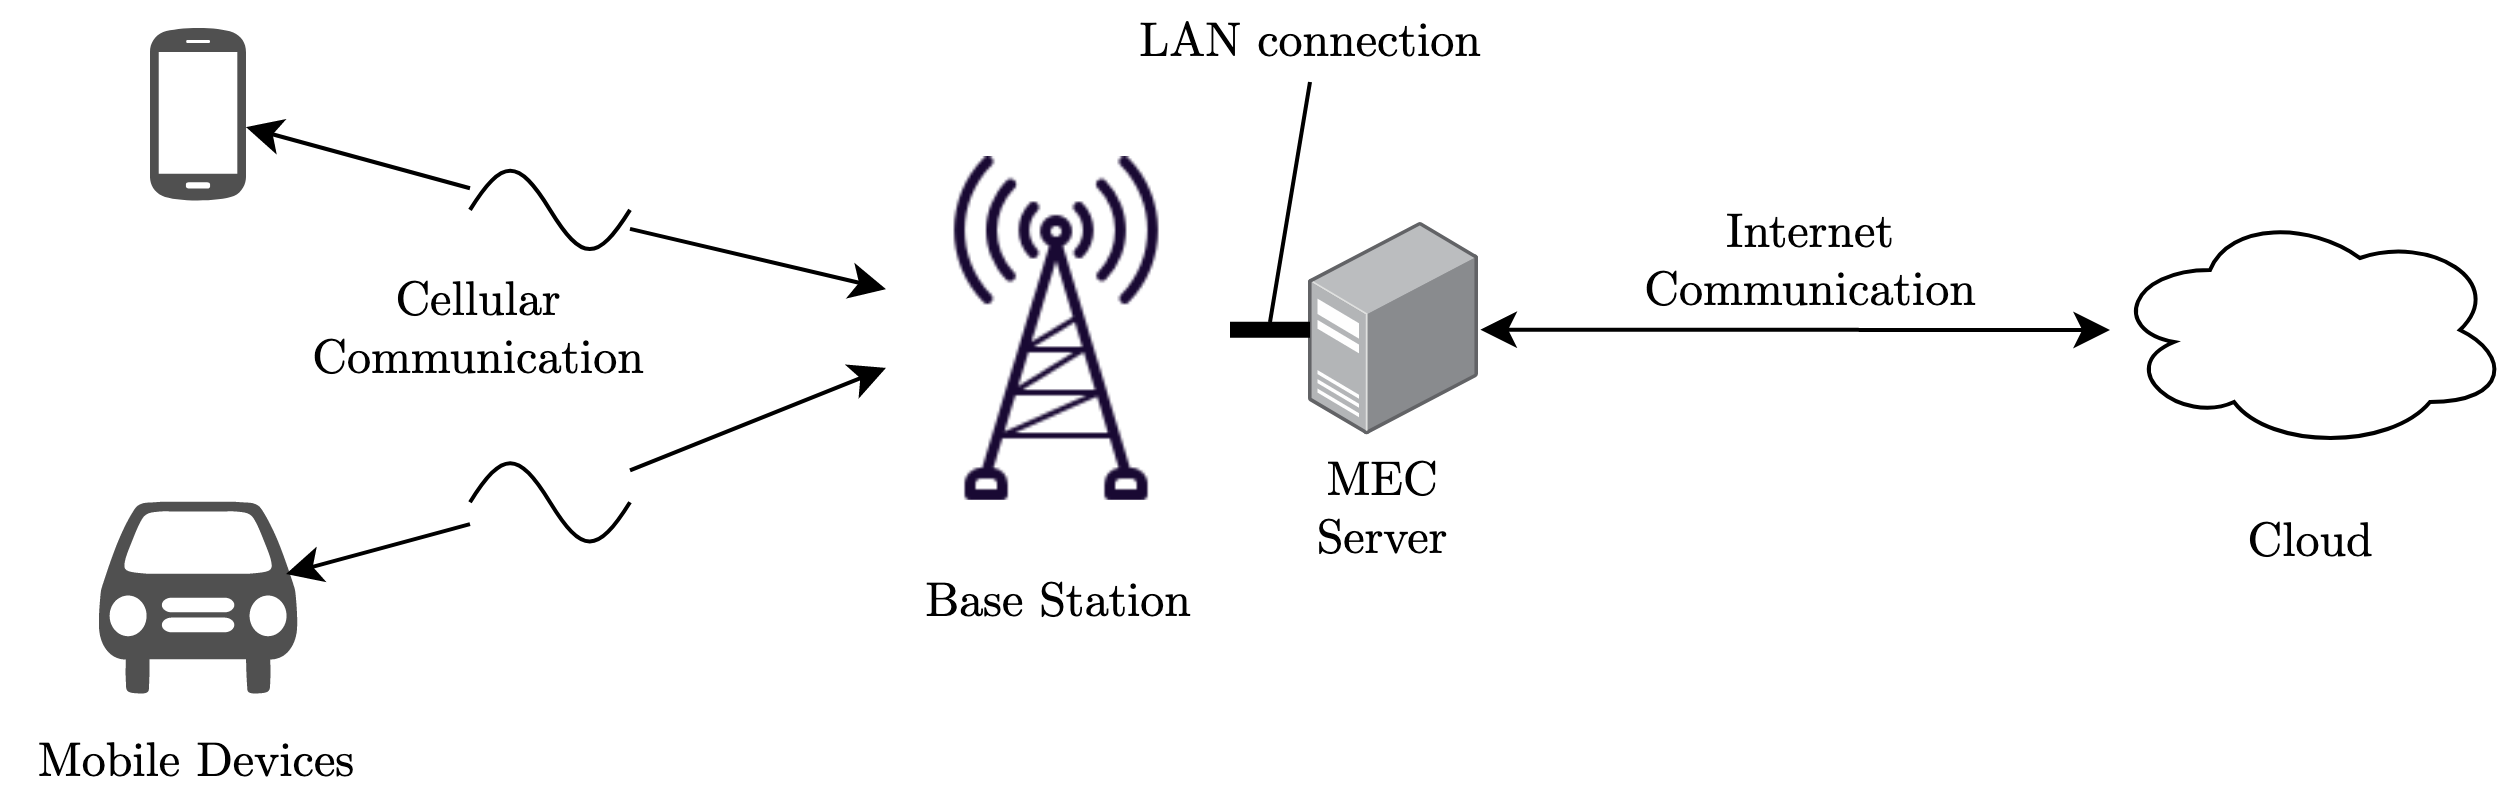
\includegraphics[scale=0.75]{chapters/architectures/figures/MEC.png}
    \caption{Diagram of MEC}
    \label{fig:MEC}
\end{figure}

\subsection{Offloading}
Figure \ref{fig:MEC} shows how MEC works on a high level. MEC will utilize the ubiquitous cellular network to offload its work. At the base station there will be a MEC server that can provide storage and computational power to the mobile devices. However, the base station servers is not as powerful as the distant cloud servers. Since the base station is just one hop away, we don't have to deal with the dynamic wide-area network. Additionally, the cellular network provides a very small delay, as base stations are relatively close by to almost everywhere where there are developed civilization. If the servers at the base station are overloaded they can send the work further to the data centres of the distant cloud or a CDN. The mobile devices can be any type of device that need storage offloading. The only requirement for this architecture is that it has a cellular or WiFi connection.

The MEC server architecture is divided into several layers that together forms three systems\cite{patel_mec_nodate}. At the bottom is the hardware layer. Over that is the virtualization layer. These two layers is part of the MEC Hosting Infrastructure Management System. Over that is the MEC Application Platform Management System which consists of a MEC virtualization manager layer and and MEC Application Platform Services layer. The virtualization manager can provide IaaS. The MEC Application Platform Services layer is an interface for the virtual machines that the applications is running on. The VMs and the apps form the Application Management Systems. Figure \ref{fig:MEC_Server} is a simplified version of the server architecture presented in \cite{patel_mec_nodate}. It shows that we can have several applications running simultaneously on the MEC Server. All the Applications run in a VM that is controlled by the MEC Application Platform Services.
\begin{figure}[t]
    \centering
    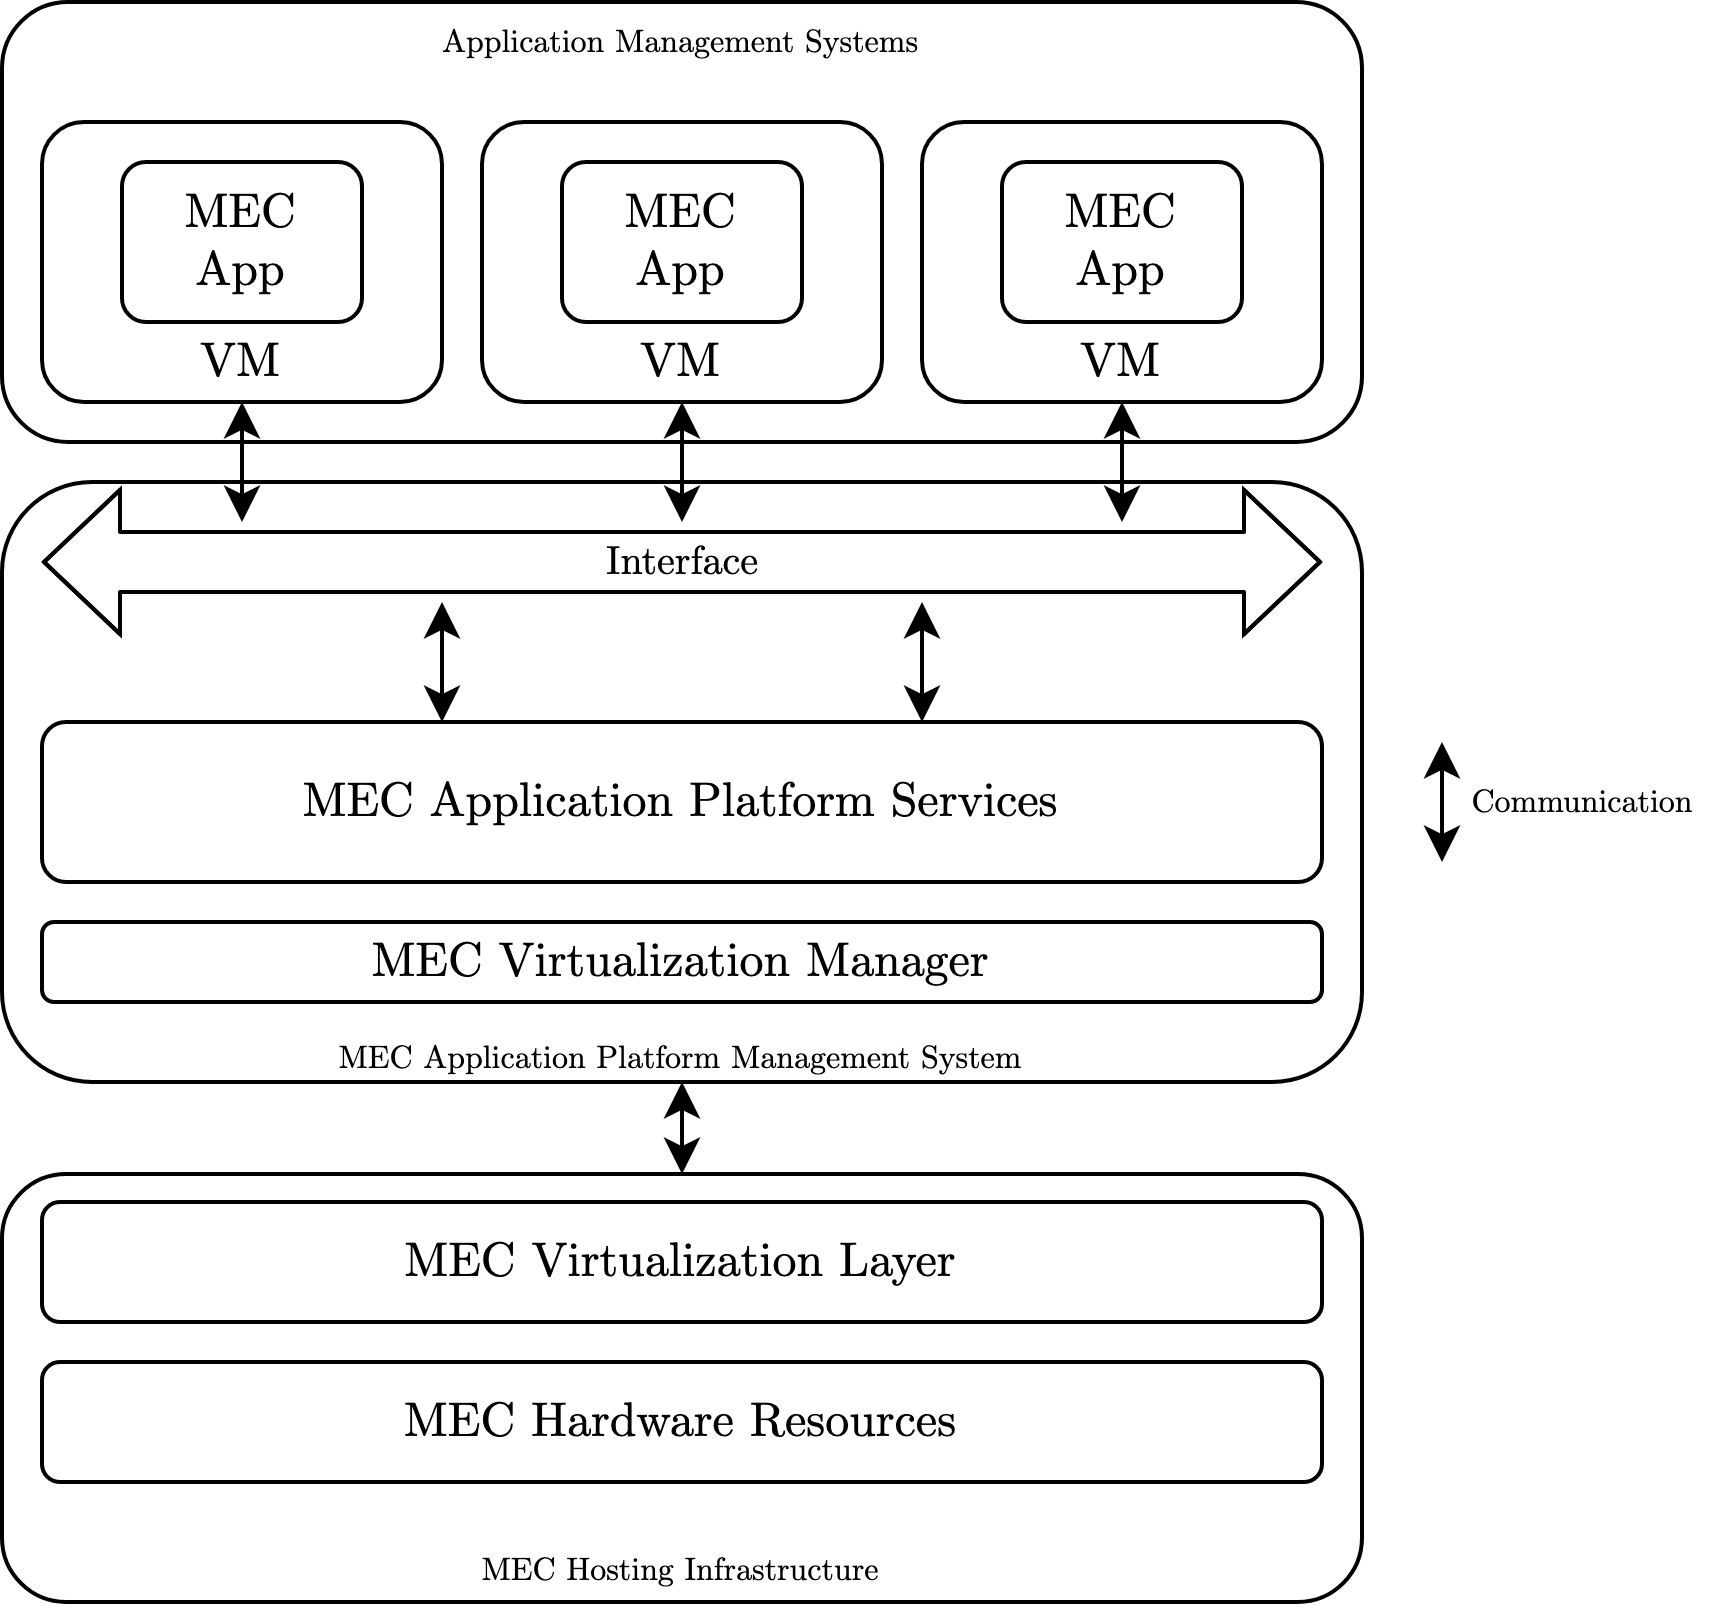
\includegraphics[scale=0.8]{chapters/architectures/figures/MEC_Server.png}
    \caption{Simplified version of the MEC Server architecture}
    \label{fig:MEC_Server}
\end{figure}

%TODO? snakke om NFV og SDN
\subsection{Network Functions Virtualization}
Network Functions Virtualization(NFV) is used in many MEC implementations\cite{patel_mec_nodate}. Networks need to run DNS, Firewall, NAT, etc to be able to run a modern network. Traditionally all of these functions have their own hardware. However, this makes infrastructure expensive, and hard to scale. NFV was introduced as a way to virtualize these functions. These functions then run on programmable switches and servers. Since they are easily controlled they are more scalable and flexible. The flexibility opens up for more possible architectures that can be deployed. For example, if we need to add extra MEC servers, instead of having extra off all the other server, it will just run through the NFV hardware, which then will take care of all the networking functions it needs. We can then easily send data to the new MEC server instead.

\subsection{Software-Defined Networking}
Software-Defined Networking(SDN) is often used together with NFV. Instead of having limiting the data layer to the hardware of switches, we run a VM on some hardware that lets networking be programmable. We can then set up rules and define were each packet should go. Since the network is now easily programmable, we can let the programmers take control of how the network is configured. The programmers can then change configuration on the fly, and therefore adapt the network to the context needed.
% In our experiments, the Emerald VM will consist of the two bottom systems, and we will focus on the application layer.

%TODO talk about HOW it is decided how much should be offloaded


%SDN er at vi har virtuelle nettverk. Slik som at vi har eget nettverk i AWS på jobben. Vi kan da definere virtuelle nettverksdrivere og interfaces osv. For eksempel ha et eget virtuellt nettverk til kun databaseting.
%https://www.cisco.com/c/en/us/solutions/software-defined-networking/sdn-vs-nfv.html

% NFV og SDN er veldig like. NFV kjører en hel VM for å kontrollere nettverket. SDN kjører bare software og består som regel kun av rules på hva pakker skal og kan gjøre.


% sjekk ut 22?, 122,121?, 161, 163
% 162!! NFV (Network Function Virtualization)
% 166 SDN(software defined networking og NFV )
% 175, 176 ICN(Information centric networking)
% 164 NFV MEC architecture for video, gaming and AR

% IN MEC we do some on the mobile and some on the MEC server. Cloudlet however, aims to do as much as possible on the server.


% ------------------------------------------------------------------------------------------

\section{Cloudlet} \label{section:architecutres_cloudlet} 
Satyanarayanan et al., proposed in their paper “The Case for VM-Based Cloudlets in Mobile Computing”\cite{satyanarayanan_case_2009} a solution to resource poverty of mobile devices and for the high latency in the Wide-Area Network(WAN). They wanted something that could fulfill the need for real-time responsiveness by having low-latency, one-hop, high-bandwidth access to a nearby \textit{Cloudlet}. They describe Cloudlets as a "data centre in a box"\cite{satyanarayanan_case_2009}. They are small computers that will run locally at each location where they are needed. All it needs is access to internet and power. An example is setting it up in a coffee shop. There it will be able to serve costumers with computation and storage if needed. All the coffee shop needs to do is plug in and configure the cloudlet. Since it is a relatively small box, it will not take much space or be in the way of costumers or employees. Having the Cloudlet so close, will help the response time stay low, as well as being predictable.

In this architecture, they focus on having as much as possible of the computation done on the nearby Cloudlet. The mobile device is just a thin client, and offloads all computation to the Cloudlet. If no Cloudlet is available, then the mobile device will try to offload to the distant cloud, or if all else fails, use its own computing power. This will heavily affect performance, especially if it has to do the work locally. However, if it detects a nearby Cloudlet, it can easily migrate the work over to it, and return to full functionality.
 
\begin{figure}[t]
    \centering
    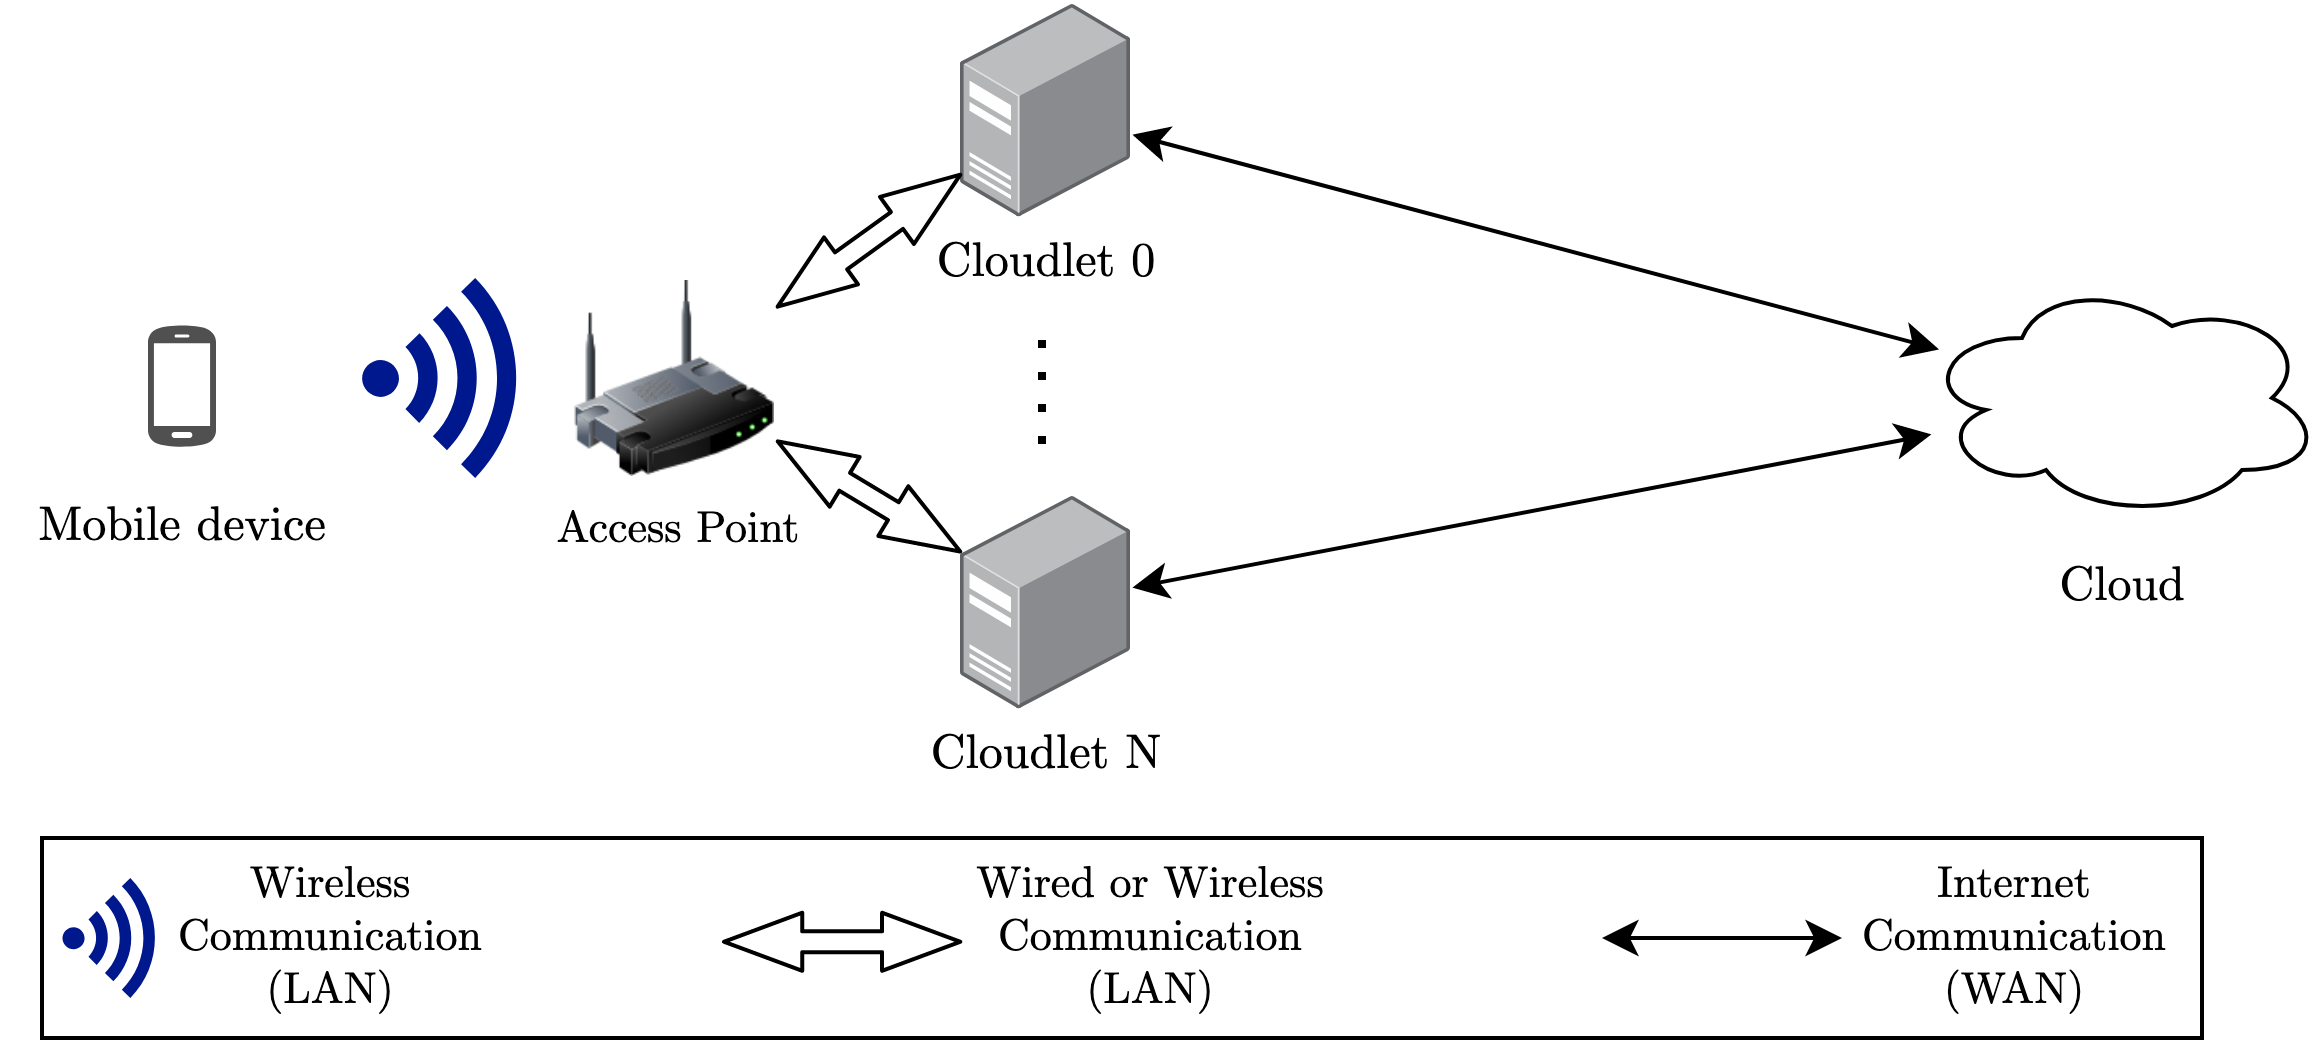
\includegraphics[scale=0.9]{chapters/architectures/figures/Cloudlet.png}
    \caption{Illustration of a simple Cloudlet connection}
    \label{fig:Cloudlet}
\end{figure}

% Husk at cloudlet kan videre overføre til distant cloud.
Figure \ref{fig:Cloudlet} shows a simple overview of how Cloudlets are connected. A mobile device will use WiFi or cellular to connect to its closest access point. The access point is further conneted to one or more Cloudlets with a LAN connection. Since they are so close in proximity of the mobile device, and on LAN, it can easily achieve just 1ms round-trip-time to the Cloudlet. In their paper, Satyanarayanan et al.\cite{satyanarayanan_case_2009} also proposes that that ideally, the Cloudlets them selves can be the access point, such that the Cloudlet is truly one-hop away, and so that they become more ubiquitous. The mobile device is usually connected to just one Cloudlet, but can easily be connected to several if needed. The Cloudlets are further connected to the distant cloud. Not shown in the figure is the case when there is no Cloudlets available. It will then connect directly to the Cloud instead of via a Cloudlet. 


\subsection{Offloading}
To simplify deployment, Cloudlets use \textit{transient customization of Cloudlet infrastructure}. Ideally it should be self managing, but it is never that easy. They want to use VMs that are fast and easy to deploy on the Cloudlets. Each time a mobile device wants to use a Cloudlet, it will send a small overhead to the server that contains enough information to start a VM that can be use to offload the work. By using VMs they ensure that creating programs for the Cloudlet is not limited to an small API or language. In other words, they let the developers decide the environment. The Cloudlet will get rid of the VM after it is finished with its use. This ensures that the Cloudlet is in the same state as before it was used.



% ------------------------------------------------------------------------------------------



\section{Google Anthos}
Google Cloud Platform(GCP) has been providing Cloud solutions since 2008. Like many other cloud providers, you can rent hosted servers on GCP. In 2019 Google announced Google Anthos, also known as just Anthos. Anthos is a way to bring GCP to the edge and on-premises\cite{noauthor_anthos_nodate}. A client can easily install Anthos software on one of their on-premises machines, and connect it to their GCP. In the GCP console, you can then control this new node in the Anthos control panel. You can then set up a cluster consisting of nodes that resides on the edge and in the data centre, and let them easily collaborate with each other. GCP will control the device that you have connected to Anthos. This ensures that you do not have to think about security. It also lets you easily manage them.

\subsection{Offloading}
Google Anthos uses Kubernetes\cite{noauthor_production-grade_nodate} to easily create distributed systems\cite{noauthor_anthos_nodate}. This means that everything that runs on the Anthos platform uses container software and middleware like Docker(see section \ref{background:docker}), and every program that runs on it is within a Docker container. Due to containerization of programs, we can easily distributed them on this platform. This enables us to easily offload work to edge nodes as well as nodes in the distant data center.
\begin{figure}[t]
    \centering
    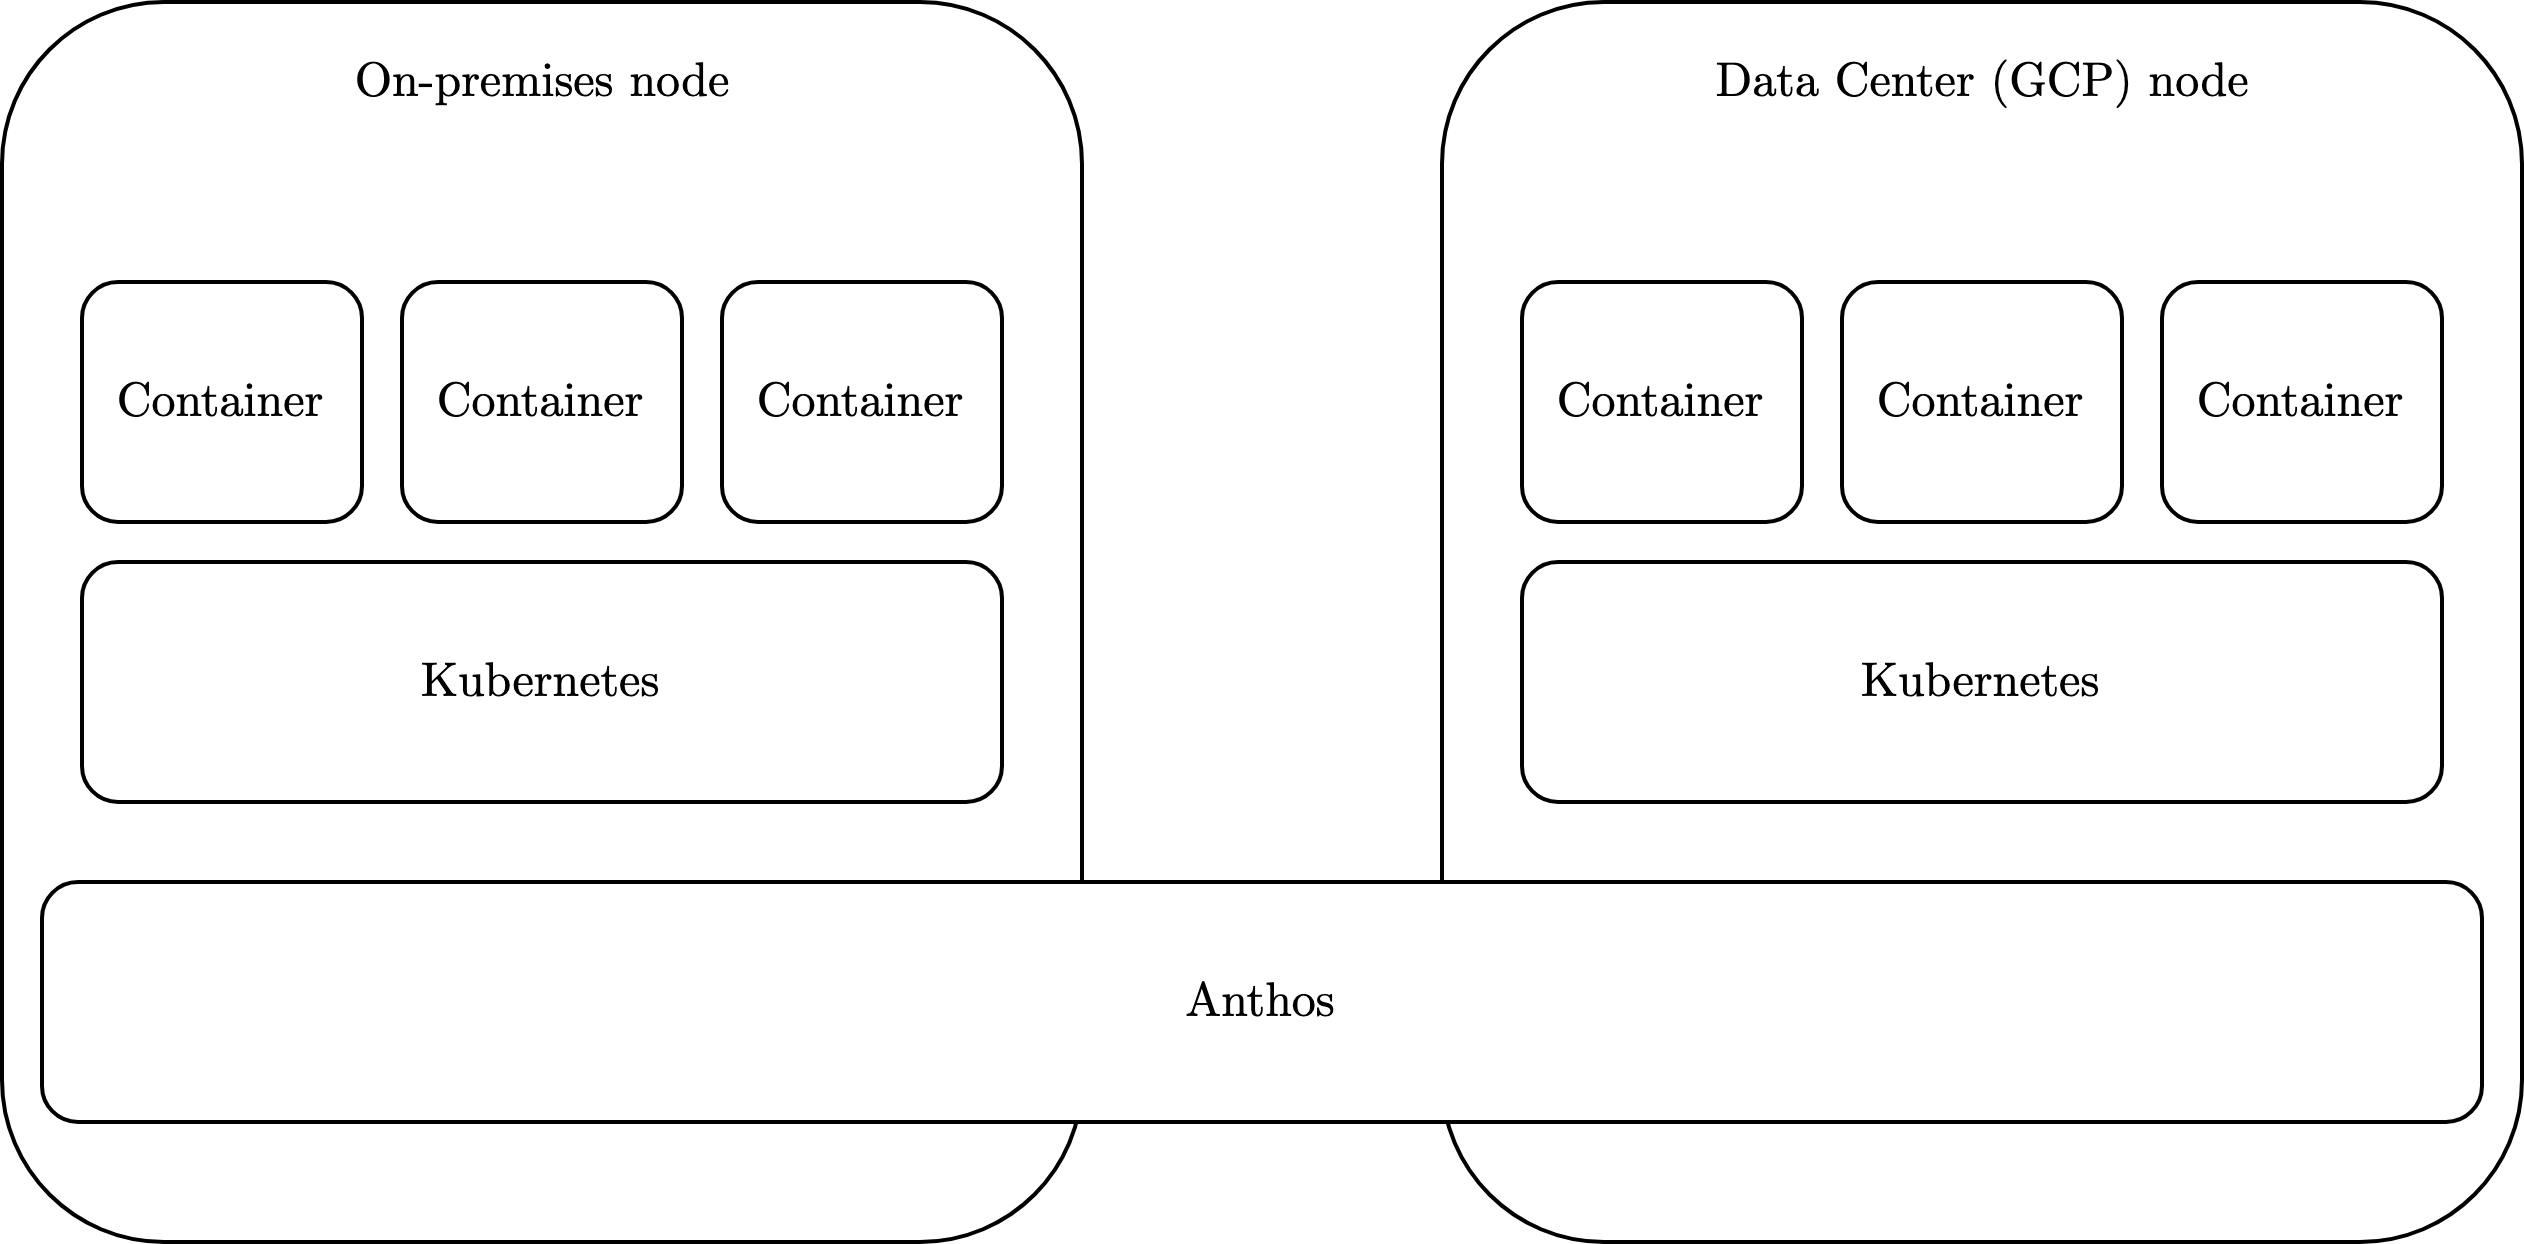
\includegraphics[scale=0.9]{chapters/architectures/figures/anthos_architecture.png}
    \caption{Illustration of a simple two nodes running on Anthos}
    \label{fig:Anthos_architecture}
\end{figure}
Figure \ref{fig:Anthos_architecture} show a simplified overview of two nodes running on Anthos. Anthos middleware runs in each node and controls a Kubernetes cluster. Zero or more containers runs on Kubernetes.
% Uses devices in your home like the chromecast or google home?
%Gir deg muligheten til å deploye on the edge, "on-premises". Veldig lik de andre
%https://cloud.google.com/anthos/docs/concepts/overview
%kanskje bare sammenligne characteristics for denne? På et vis, bare droppe å bruke programmet fordi det uansett blir så likt.


% -------------------------------------------------------------------------------

\section{Amazon Cloudfront}
Amazon Web Services (AWS) provides Amazon Cloudfront as a solution for latency-aware applications\cite{noauthor_production-grade_nodate}. Amazon Cloudfront is a CDN service that lets you integrate other important AWS services at the edge. This lets you easily provide storage and computation at the edge. Additionally, you get the safety that is already integrated in the services that AWS provides. 

\subsection{Offloading}
Within Amazon Cloudfront they provide a service called Lambda@Edge. AWS Lambda is a serverless service that lets you run small functions in the cloud so that you do not need a whole server, for a small piece of code. Also, it lets you easily scale if need be. Lambda@Edge lets you put these Lambda functions on the edge, and therefore closer to the user. It then lets you easily connect to their database services to provide storage. This storage can also be at the edge if its needed. When storage offloading is needed, you just call a Lambda function that is placed at the edge. You will then get a really fast response, as the computation happens geographically close to you.



% ------------------------------------------------------------------------------

\section{Akamai}
Akamai is a company which specializes on bringing content closer to the edge by using Content Delivery Networks. It has become widely popular, and a significant portion of the web moves through an Akamai device. They will have servers directly at the ISP’s so clients are just one “network hop” away from their servers. Akamai\cite{noauthor_exceptional_nodate} claims \say{85\% of the world’s Internet users are within a single “network hop” of an Akamai edge server.}. They also claim to handle 15-30\% of the world's web traffic. Companies pay Akamai to cache videos and web pages closer to the user. This helps improve latency and stability, as interaction through Wide-Area Network is minimized. 

\begin{figure}[t]
    \centering
    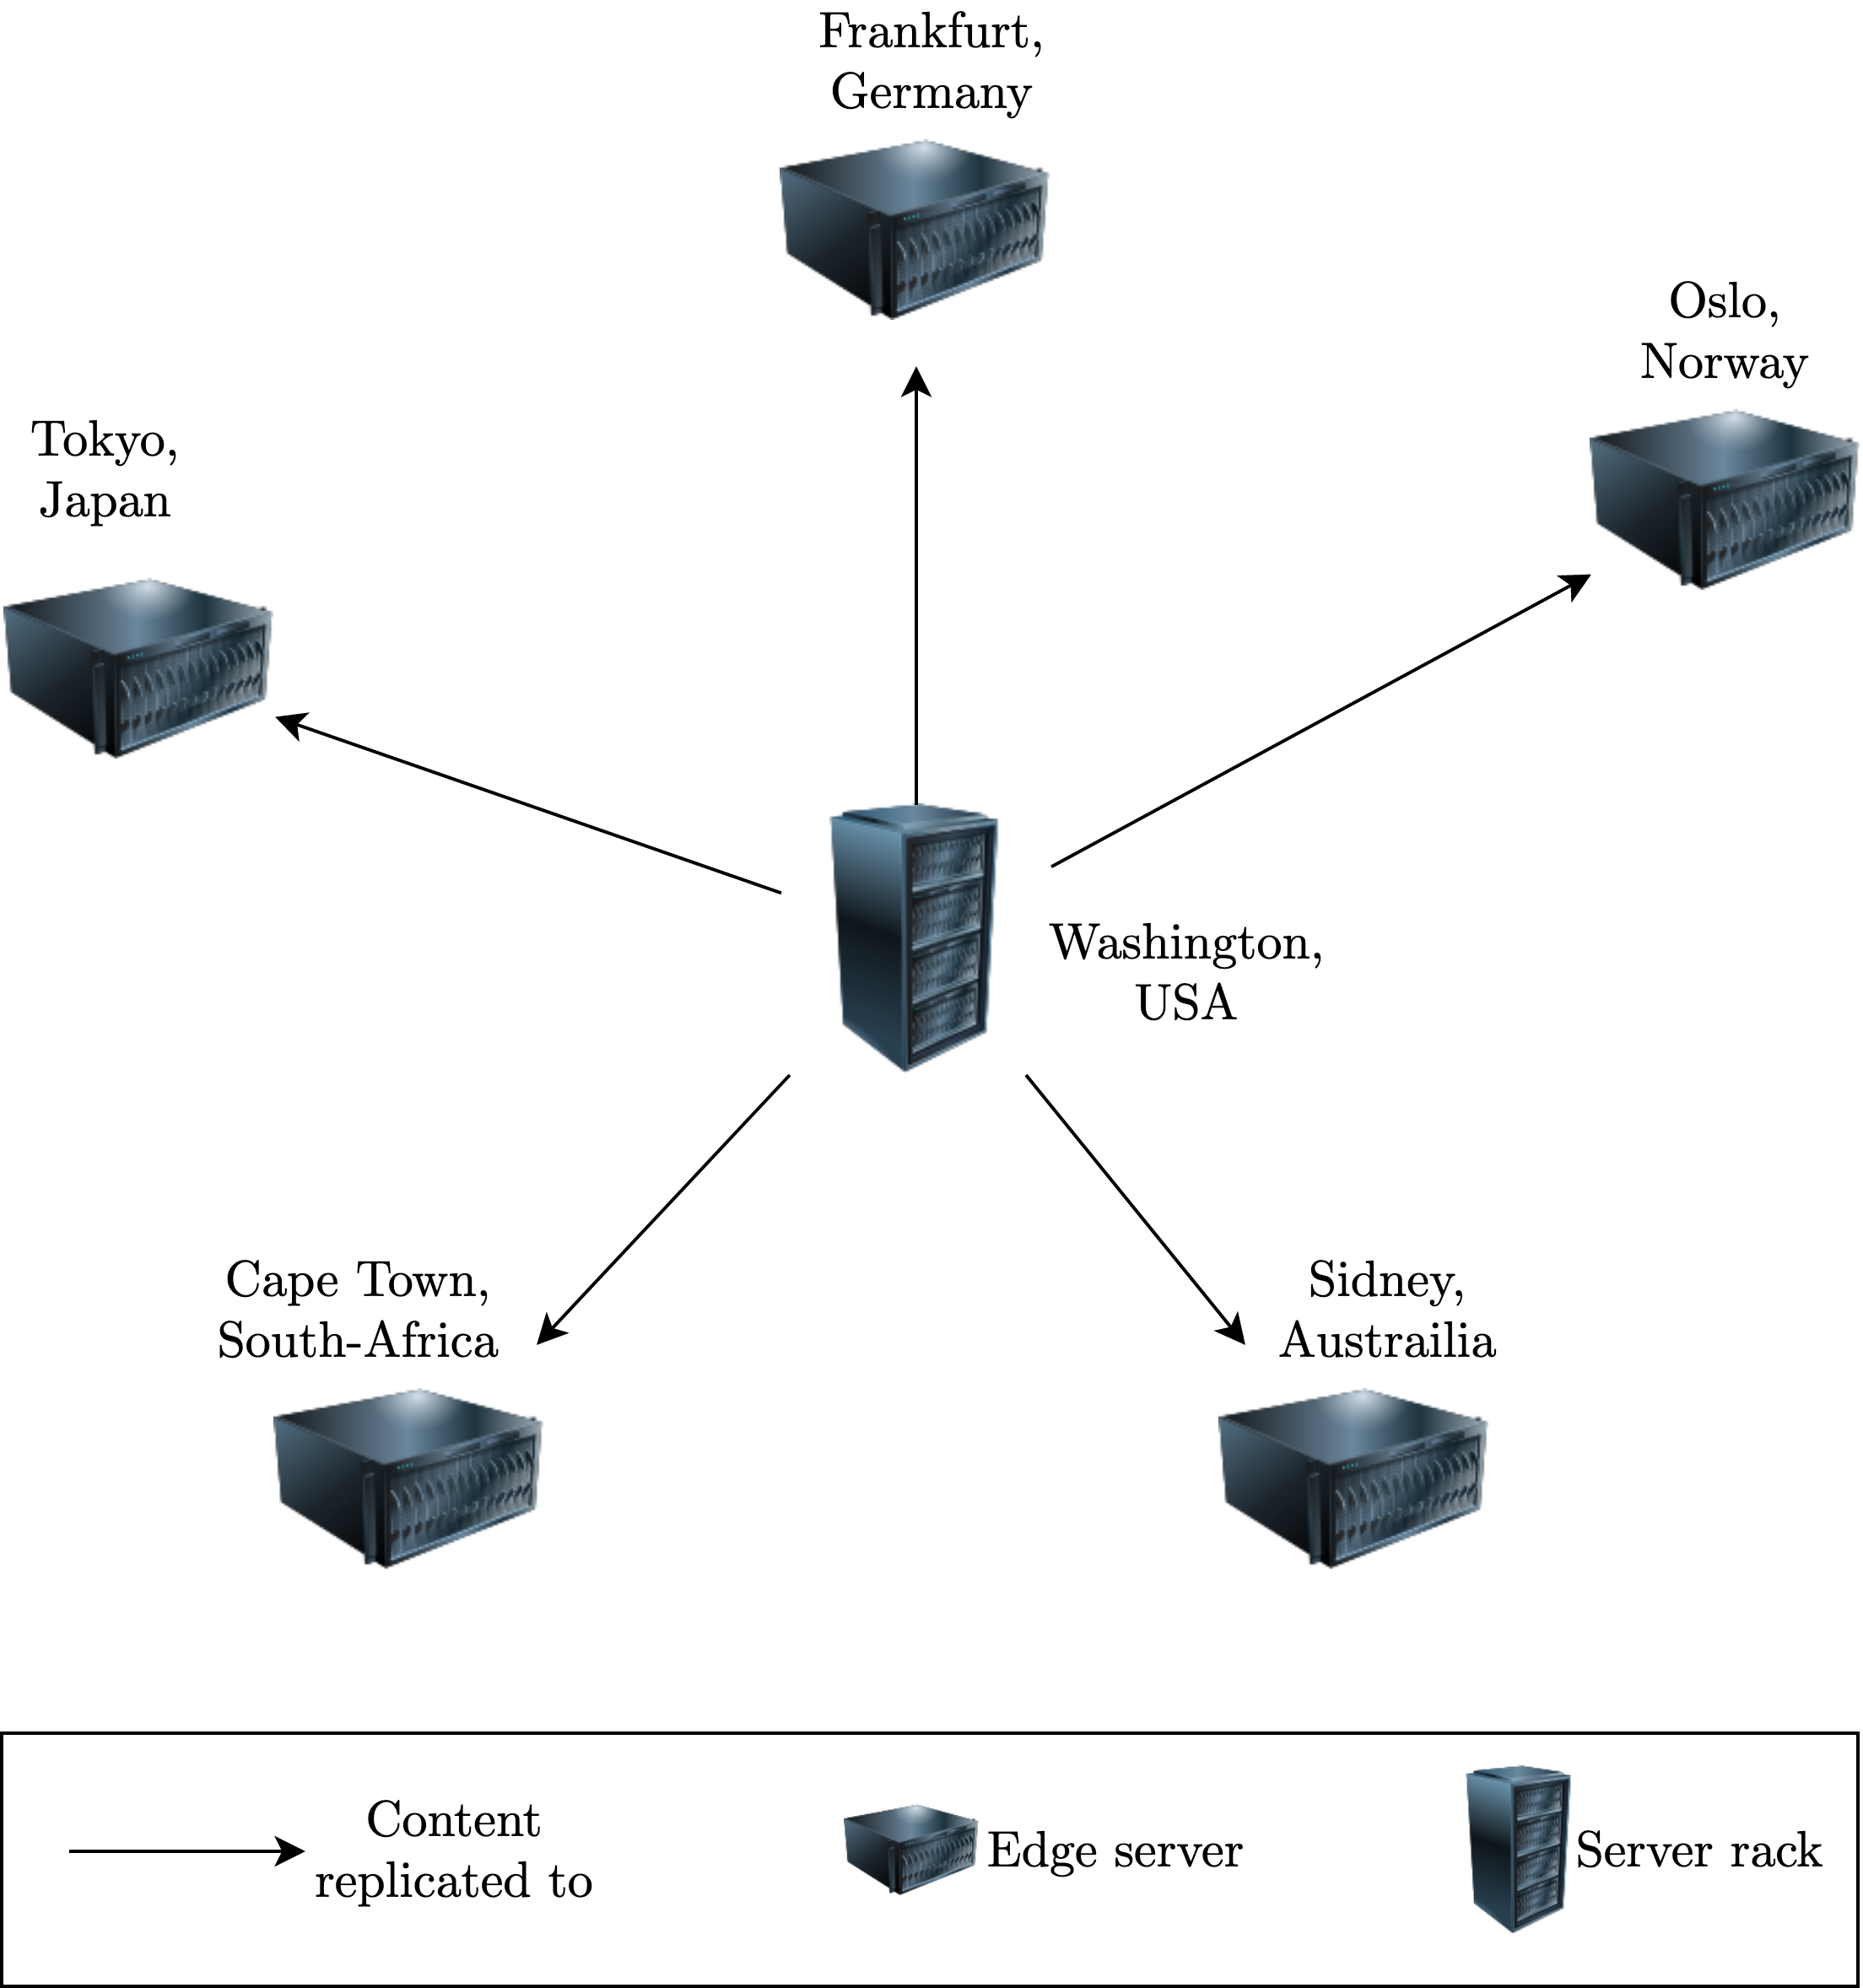
\includegraphics[scale=0.8]{chapters/architectures/figures/akamai_dist.png}
    \caption{Simplified Illustration of replication in Akamai CDN}
    \label{fig:Akamai_cdn}
\end{figure}

Figure \ref{fig:Akamai_cdn} shows how content is replicated across the world. A big server rack might be in Washington an contains the web content for a page there. If we were to get this page from the other side of the world in Norway, then there will be significant latency and instability when trying to retrieve the content. The server will therefore benefit from replicating the page to an Akamai server in Oslo, Norway. Then when someone in Norway tries to retrieve the page, it will instead get it from the Edge server that is geographically close to the end user. However should one of the edge servers be overloaded or fail, then it will let you get content from the original server in Washington. 




\section{Summary}
In this chapter we have presented several architectures that focuses on mitigating latency. We have presented how they work, and how they are setup. We have focused on presenting how they offload work or storage where applicable. 